\documentclass[10pt]{article}

\usepackage[margin=0.85in]{geometry}
\usepackage{graphicx}
\usepackage{amsmath}
\usepackage{amssymb}
\usepackage{listings}
\usepackage{xcolor}
\usepackage{tikz}
\usepackage{booktabs}
\usepackage{caption}
\usepackage{float}
\usepackage{url}
\usepackage{hyperref}
\usepackage{enumitem}

\setlist{nosep,leftmargin=*}
\setlength{\parskip}{2pt plus 1pt}
\setlength{\textfloatsep}{6pt}
\setlength{\floatsep}{6pt}
\setlength{\intextsep}{4pt}
\setlength{\abovecaptionskip}{4pt}
\setlength{\belowcaptionskip}{2pt}

\usetikzlibrary{shapes,arrows,positioning,calc}

\definecolor{lightblue}{RGB}{173,216,230}

\lstset{
  basicstyle=\ttfamily\footnotesize,
  keywordstyle=\color{blue},
  commentstyle=\color{gray},
  stringstyle=\color{red},
  breaklines=true,
  postbreak=\mbox{\textcolor{red}{$\hookrightarrow$}\space},
  language=C++,
  showstringspaces=false,
  aboveskip=4pt,
  belowskip=4pt
}

\lstdefinelanguage{MLIR}{
  morekeywords={gpu,module,func,binary,object,target,select_object,runtime_select,nvvm,rocdl,xevm,chip},
  morecomment=[l]{//},
  morestring=[b]"
}

\title{\vspace{-1.5em}Runtime Variant Selection in LLVM's GPU Offload Stack:\newline
  Metadata, Measurement, and Mechanism\vspace{-0.5em}}

\author{Akash \\
  IIT Patna, CERN GSoC Alumnus, vLLM Contributor}

\date{EuroLLVM Developers' Meeting, Dublin 2026\vspace{-1em}}

\begin{document}

\maketitle

\begin{abstract}
Deploying ML kernels across heterogeneous GPU clusters requires separate builds per vendor---CERN HEP-CCE manages 80 build configurations for mixed A100/V100, MI250X, and CPU targets alone.
LLVM's \texttt{OffloadBinary} format carries multiple device images in a single fat binary, but the runtime selects the first compatible image and stops, with no mechanism to rank alternatives.
We address this gap with three contributions.
First, a backward-compatible metadata vocabulary: five new \texttt{OffloadBinary} string keys expressing minimum hardware requirements and variant priority.
Second, the first published layer-by-layer latency decomposition of LLVM's GPU offload path, measured on a GTX~1650, showing cold initialization dominates at 89.6\% of the 40\,$\mu$s dispatch budget.
Third, \texttt{\#gpu.runtime\_select}, an MLIR attribute that consumes this metadata to select the best-compatible image at load time, adding only 3\,ns of amortized selection overhead.
Together, these contributions establish the mechanism for single-binary multi-vendor GPU deployment within LLVM's existing offload infrastructure.
\end{abstract}

\section{Introduction}

Since August 2025 (PR~\#148286), MLIR's \texttt{gpu-module-to-binary} pass compiles a single source to NVIDIA (\texttt{\#nvvm.target}), AMD (\texttt{\#rocdl.target}), and Intel (\texttt{\#xevm.target}).
The \texttt{OffloadBinary} fat-binary format (D122069, 2022) carries all device images in one container.

Yet the runtime has not caught up.
\texttt{parseOffloadBinary} (PR~\#186088) selects the \textit{first} image whose triple and architecture match, then stops.
No mechanism exists to express image quality tiers or select among multiple compatible options.

This gap matters today.
HEP-CCE at CERN maintains 80 separate build configurations for heterogeneous GPU clusters (A100/V100 + MI250X + CPU).
vLLM maintains separate NVIDIA and AMD codepaths.
Cloud containers face unknown GPU models at build time.
A single fat binary with runtime selection eliminates all three workarounds.

We propose three contributions: a metadata vocabulary (C1) describing what each image requires, a layer-by-layer latency decomposition (C2) measuring the cost budget, and a compiler attribute design (C3) showing how the metadata enables selection.

\section{Background}

The compilation pipeline from \texttt{gpu.module} to fat binary is complete:

\begin{lstlisting}[language=MLIR]
gpu.binary @kernels <#gpu.select_object<0>> [
  #gpu.object<#nvvm.target<chip = "sm_75">, bin = "...">,
  #gpu.object<#rocdl.target<chip = "gfx90a">, bin = "...">,
  #gpu.object<#xevm.target<chip = "pvc">, bin = "...">
]
\end{lstlisting}

\texttt{\#gpu.select\_object} is the only implementation of the offloading translation interface---it locks in a single image \textit{at compile time} by index or static match.
RFC~\#88170 separates the container (``\texttt{gpu.binary} holds N objects'') from the policy slot (``who decides which one runs?'').
The policy slot is vacant.

The runtime consumer hook exists: \texttt{isMetadataCompatible()} (PR~\#185663, merged March 2026) filters images during parse.
Today \texttt{OffloadBinary} carries only \texttt{triple} and \texttt{arch} per image.
\textbf{The consumer exists. The vocabulary does not.}

\section{Contributions}

\subsection{Contribution 1: OffloadBinary Metadata Vocabulary}

We propose five new string keys in two tiers.

\subsubsection{Tier 1: MUST Keys (Runtime Rejects if Violated)}

\begin{center}
\footnotesize
\begin{tabular}{llp{2.5cm}l}
  \toprule
  Key & Type & Example & Semantics \\
  \midrule
  \texttt{min\_sm} & uint & \texttt{"75"} & Min CUDA SM. Reject if device $<$ value. \\
  \texttt{min\_gfx} & arch:family & \texttt{"gfx90a:cdna2"} & Min AMD GFX within ISA family. \\
  \texttt{requires\_features} & comma-list & \texttt{"tensor\_core\_nv,bf16"} & Named capability tokens. \\
  \bottomrule
\end{tabular}
\normalsize
\end{center}

Tokens are vendor-specific by design (\texttt{tensor\_core\_nv}, \texttt{mfma\_amd}) to prevent false cross-vendor capability matches.

\subsubsection{Tier 2: MAY Keys (Ranking, Not Gating)}

\begin{center}
\footnotesize
\begin{tabular}{llll}
  \toprule
  Key & Type & Example & Semantics \\
  \midrule
  \texttt{variant\_priority} & uint & \texttt{"10"} & Higher = preferred among compatible. \\
  \texttt{variant\_tag} & string & \texttt{"optimized"} & Human-readable label. \\
  \bottomrule
\end{tabular}
\normalsize
\end{center}

These extend \texttt{isMetadataCompatible()} without format version bump or ABI break:

\begin{lstlisting}[language=C++]
bool isMetadataCompatible(image, device) {
  if (image.Triple != device.Triple) return false;
  if (!areArchsCompatible(image.Arch, device.Arch))
    return false;
  if (auto minSm = image.getString("min_sm"))
    if (parseSmFromArch(device.Arch) < stoul(*minSm))
      return false;
  if (auto features = image.getString("requires_features"))
    for (auto &tok : split(*features, ','))
      if (!device.hasCapability(tok)) return false;
  return true;
}
\end{lstlisting}

\textbf{Backward compatibility:} Missing keys = no constraint. Old runtimes ignore unknown keys.

\subsection{Contribution 2: Dispatch Layer Decomposition}

We decompose the CUDA driver API dispatch path on a GTX 1650 (Turing, sm\_75) using a null kernel (1 thread, 0 shared memory) compiled to a 4328-byte CUBIN.
All measurements use CPU-pinned execution (\texttt{taskset -c 0}).
Reported values are cross-run medians over 3 independent runs.
Cold-path: \texttt{execve} per trial (100 trials/run, clean address space).
Hot-path: warm with 100 discarded iterations, measure 10,000/run.

\subsubsection{Results}

\textbf{Cold-path layer decomposition} (GTX 1650, null kernel, CUBIN, pinned 3-run medians from \texttt{bench\_layers})\footnote{Cold-path measurement includes process startup, \texttt{dlopen}, \texttt{cuInit}, and \texttt{cuCtxCreate} in addition to \texttt{cuModuleLoadData}. The warm-path measurement (9.6\,$\mu$s) isolates the module-load cost.}:

\begin{center}
\footnotesize
\begin{tabular}{llrrrr}
  \toprule
  Layer & Operation & Median & p99 & CV\% & \% of Total \\
  \midrule
  2 & Cold init + cuModuleLoadData\textsuperscript{$\dagger$} & $35{,}953\,\text{ns}$ & $59{,}602\,\text{ns}$ & $0.7$ & $89.6\%$ \\
  4 & cuLaunchKernel (submit) & $1{,}650\,\text{ns}$ & $3{,}011\,\text{ns}$ & $1.0$ & $4.1\%$ \\
  5 & cuStreamSynchronize & $2{,}454\,\text{ns}$ & $3{,}601\,\text{ns}$ & $0.5$ & $6.1\%$ \\
  3 & cuModuleGetFunction & $63\,\text{ns}$ & $90\,\text{ns}$ & $9.1$ & ${\sim}0.2\%$ \\
  \midrule
  & Cold end-to-end (L2+L3+L4+L5) & \multicolumn{3}{c}{${\sim}40{,}120\,\text{ns}$} & \textbf{100\%} \\
  \bottomrule
\end{tabular}
\normalsize
\end{center}

{\footnotesize\textsuperscript{$\dagger$}Full cold path via \texttt{execve}: includes process creation, \texttt{dlopen(libcuda.so.1)}, \texttt{cuInit}, \texttt{cuDeviceGet}, \texttt{cuCtxCreate}, and \texttt{cuModuleLoadData}. CV\% = coefficient of variation across 3 pinned runs (cross-run median).
95\% CI from 3-run cross-run medians ($t_{0.025,2}{=}4.303$): cold init $36.0 \pm 0.6$\,\textmu{}s, hot-path $4.1 \pm 0.01$\,\textmu{}s.}

\textbf{Hot-path dispatch floor} (cuLaunchKernel + cuStreamSynchronize, $n{=}10{,}000$/run, 3 pinned runs):

\begin{center}
\footnotesize
\begin{tabular}{ll}
  \toprule
  Metric & Value \\
  \midrule
  Median (launch + sync) & $4{,}104\,\text{ns}$ (CV~0.1\%) \\
  cuLaunchKernel p99 & $3{,}011\,\text{ns}$ \\
  cuStreamSynchronize p99 & $3{,}601\,\text{ns}$ \\
  \bottomrule
\end{tabular}
\normalsize
\end{center}

\textbf{Selection overhead} (two distinct measurements):

\begin{center}
\footnotesize
\begin{tabular}{lllr}
  \toprule
  System & Operation & Value & CV\% \\
  \midrule
  libkdl prototype (MTB format) & \texttt{kdl\_select} cold & $52.6\,\mu\text{s}$ & $4.3$ \\
  OffloadBinary (\texttt{runtime\_select\_poc}) & dispatch-table lookup & $3\,\text{ns}$ & $0.0$ \\
  \bottomrule
\end{tabular}
\normalsize
\end{center}

{\footnotesize The libkdl prototype uses a custom MTB bundle format, not OffloadBinary---the 52.6\,$\mu$s measures its hash-table selection path ($n{=}1{,}000$/run, 3 pinned runs).
The 3\,ns figure is the amortized steady-state cost of dispatch-table lookup in the proposed LLVM design (OffloadBinary metadata scan, $100{,}000$ iterations, 3 pinned runs).
\textbf{The 3\,ns OffloadBinary lookup is the number relevant to the proposed \texttt{\#gpu.runtime\_select} design.}
Both add $<$\,1\% overhead for kernels $\geq$\,10\,ms (typical production ML).}

\subsubsection{Latency Decomposition Visualization}

\begin{figure}[H]
  \centering
  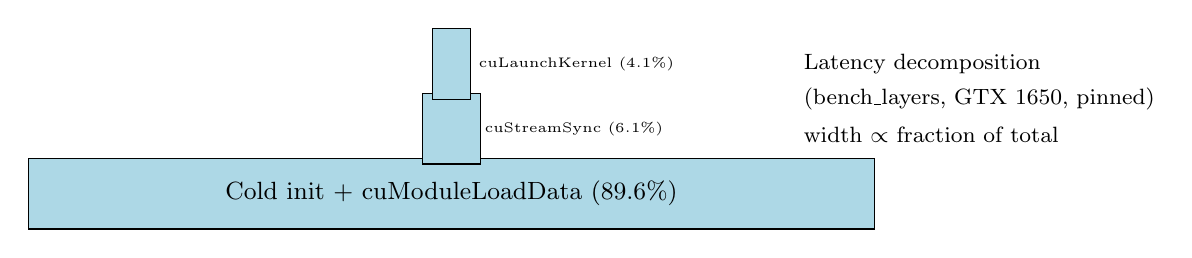
\begin{tikzpicture}[scale=0.75]
    % Latency decomposition chart: bottom bar = widest (dominant layer).
    % Base width 12cm = 100% of cold-dispatch latency.
    \node[draw, rectangle, minimum width=10.75cm, minimum height=0.9cm, fill=lightblue] at (0, 0)
      {\small Cold init + cuModuleLoadData ($89.6\%$)};
    \node[draw, rectangle, minimum width=0.73cm, minimum height=0.9cm, fill=lightblue] at (0, 1.1)
      {};
    \node[anchor=west] at (0.40, 1.1) {\tiny cuStreamSync ($6.1\%$)};
    \node[draw, rectangle, minimum width=0.49cm, minimum height=0.9cm, fill=lightblue] at (0, 2.2)
      {};
    \node[anchor=west] at (0.30, 2.2) {\tiny cuLaunchKernel ($4.1\%$)};
    % Annotation
    \node[anchor=west] at (5.8, 2.2) {\footnotesize Latency decomposition};
    \node[anchor=west] at (5.8, 1.6) {\footnotesize (bench\_layers, GTX 1650, pinned)};
    \node[anchor=west] at (5.8, 1.0) {\footnotesize width $\propto$ fraction of total};
  \end{tikzpicture}
  \caption{Cold-path latency decomposition chart (pinned 3-run medians). Bar width proportional to fraction of total cold-dispatch latency (${\sim}40.1\,\mu$s). Hot-path floor: 4.1\,$\mu$s (L4+L5 only).}
\end{figure}

\subsection{Contribution 3: Design Sketch --- \texttt{\#gpu.runtime\_select}}

\textbf{Status: Design only. Zero lines of MLIR C++ exist.}

The new attribute implements \texttt{OffloadingLLVMTranslationAttrInterface}:

\begin{lstlisting}[language=MLIR]
gpu.binary @kernels <#gpu.runtime_select<
    strategy = "rank_by_priority", fallback = "cpu">> [
  #gpu.object<#nvvm.target<chip = "sm_75">, bin = "...">,
  #gpu.object<#rocdl.target<chip = "gfx90a">, bin = "...">,
  #gpu.object<#nvvm.target<chip = "sm_90">, bin = "...">
]
\end{lstlisting}

\texttt{embedBinary()} emits: (1)~N LLVM global constants (one per object); (2)~a dispatch table: \texttt{\{vendor\_id, blob\_ptr, size\}}; (3)~a vendor-detection stub in \texttt{global\_ctors} via \texttt{dlopen}-probed \texttt{cuInit}/\texttt{hipInit}/\texttt{zeInit}; (4)~a \texttt{@\{symName\}\_module\_ptr} global populated at constructor time.
\texttt{launchKernel()} is identical to \texttt{SelectObjectAttr}---\textbf{zero hot-path overhead} after one-time selection.

\textbf{Why MLIR and not liboffload?}
liboffload explicitly excludes selection policy (RFC discourse.llvm.org/t/74302); it provides mechanism, not policy.
The analogy is direct: LLVM emits IFunc resolvers at compile time for CPU \texttt{target\_clones}; \texttt{\#gpu.runtime\_select} does the same for GPU binaries.

\subsubsection{Known Design Issues}

\begin{enumerate}
  \item \textbf{Static initialization ordering:} \texttt{global\_ctors} vendor-detection runs before \texttt{main}. CUDA contexts created this early may conflict with user \texttt{cuCtxCreate} calls.
  \item \textbf{dlopen + sanitizer interaction:} AddressSanitizer intercepts \texttt{dlopen}. Vendor-detection stubs must be sanitizer-aware or gated behind a check.
\end{enumerate}

\section{Prototype Validation}

libkdl (${\sim}5100$ LOC, C) implements the runtime mechanics: vendor detection via \texttt{dlopen}, dispatch table construction, capability-based selection, and module loading via \texttt{cuModuleLoadData}/\texttt{hipModuleLoadData}.
The prototype uses a custom MTB format, not \texttt{OffloadBinary}; the two share zero code.

\begin{center}
\footnotesize
\begin{tabular}{llp{3.5cm}}
  \toprule
  kdl.c Component & Lines & LLVM Equivalent \\
  \midrule
  \texttt{kdl\_discover\_cuda()} & 551--596 & Vendor detection (dlopen cuInit) \\
  \texttt{kdl\_contract\_matches()} & 1003--1005 & \texttt{isMetadataCompatible()} \\
  \bottomrule
\end{tabular}
\normalsize
\end{center}

Hardware validated: GTX 1650 (full dispatch path) and CPU fallback. AMD tested via mocked HIP entry points only.

\section{Related Work}

IREE HAL is the closest full-stack solution with module-level dispatch, but its developers have not yet addressed ranked image selection (issues \#12230, \#15334). In LLVM's own offload stack, PR~\#186088 explicitly defers ranked selection to a follow-up.
CPU function multi-versioning via IFunc resolvers is the structural precedent: compile-time emission of runtime selection logic.
chipStar provides CUDA-on-OpenCL portability but not ranked variant selection.
HetGPU~\cite{hetgpu} achieves cross-vendor binary portability through runtime IR translation, complementary to our AOT selection approach.
KernelEvolve~\cite{kernelevolve} validates multi-target kernel generation in production at Meta; our work addresses the runtime dispatch step that follows generation.
Our proposal extends the IFunc pattern to GPU binaries, adding a standard metadata vocabulary that LLVM currently lacks.

\section{Conclusion and Upstream Path}

The metadata vocabulary (C1) standardizes image requirements.
The latency decomposition (C2) measures the dispatch budget.
The runtime-select design (C3) shows how MLIR consumes the metadata.

\textbf{Upstream path:}
(1)~RFC on Discourse for metadata vocabulary;
(2)~header constants in \texttt{OffloadBinary.h} (${\sim}30$ LOC);
(3)~extend \texttt{isMetadataCompatible()} (${\sim}40$ LOC);
(4)~AMDGPU/NVPTX writers emit \texttt{min\_gfx}/\texttt{min\_sm} (${\sim}60$ LOC each);
(5)~\texttt{\#gpu.runtime\_select} TableGen + \texttt{RuntimeSelectAttr.cpp} (${\sim}600$ LOC), pending RFC~\#88170.
All steps after (1) are independent.

\section*{References}

\bibliographystyle{unsrt}
\begin{thebibliography}{99}

\bibitem{taxbreak}
Vellaisamy, P., Tripathi, S., Natarajan, V., et al.
\emph{TaxBreak: Unmasking the Hidden Costs of LLM Inference Through Overhead Decomposition}.
arXiv:2603.12465, 2026.

\bibitem{pygraph}
Ghosh, A., Nayak, A., Panwar, A., Basu, A.
\emph{PyGraph: Robust Compiler Support for CUDA Graphs in PyTorch}.
arXiv:2503.19779, 2025.

\bibitem{rfc88170}
Mora, F.
\emph{RFC: Cleaning the GPU Dialect}.
LLVM Discourse, September 2025.
\url{https://discourse.llvm.org/t/88170}

\bibitem{pr186088}
Duran, A.
\emph{[OFFLOAD] Generalize support for OffloadBinary images}.
GitHub PR~\#186088, LLVM Project, March 2026.

\bibitem{pr185663}
Duran, A.
\emph{[OFFLOAD] Add interface to extend image validation}.
GitHub PR~\#185663, LLVM Project. Merged March 2026.

\bibitem{pr148286}
Lee, S.I.
\emph{[MLIR][GPU][XeVM] Add XeVM target and XeVM dialect integration tests}.
GitHub PR~\#148286, LLVM Project. Merged August 2025.

\bibitem{hetgpu}
Zhao, Y., et al.
\emph{HetGPU: The Pursuit of Making Binary Compatibility Towards GPUs}.
arXiv:2506.15993, 2025.

\bibitem{universalgpuisa}
Cross-vendor analysis.
\emph{Toward a Universal GPU Instruction Set Architecture: A Cross-Vendor Analysis of Hardware-Invariant Computational Primitives in Parallel Processors}.
arXiv:2603.28793, 2026.

\bibitem{kernelevolve}
Meta Platforms.
\emph{KernelEvolve: Adaptive Kernel Generation for Heterogeneous Hardware}.
ISCA 2026. arXiv:2512.23236.

\bibitem{adaptivecpp}
Alpay, A., Heuveline, V.
\emph{Adaptivity in AdaptiveCpp: Optimizing Performance by Leveraging Runtime Information During JIT-Compilation}.
IWOCL 2025.

\end{thebibliography}

\end{document}
